\documentclass[12pt,a4paper]{article}
\usepackage{termpaper}
\usepackage[utf8]{inputenc}
\usepackage{graphicx}
\usepackage{listings}
\usepackage{xcolor}
\usepackage{cleveref}
\usepackage{filecontents}
\usepackage{minted}
\usepackage{url}

\definecolor{lstcolor}{rgb}{0.95,0.95,0.95}

\lstdefinestyle{customc}{
  belowcaptionskip=1\baselineskip,
  breaklines=true,
  frame=L,
  xleftmargin=\parindent,
  language=C,
  showstringspaces=false,
  basicstyle=\ttfamily\scriptsize,
  keywordstyle=\bfseries\color{green!40!black},
  commentstyle=\itshape\color{purple!40!black},
  identifierstyle=\color{blue},
  stringstyle=\color{orange},
  tabsize=2
}
\lstset{escapechar=@,style=customc}

\newminted{c}{tabsize=2,fontsize=\footnotesize,bgcolor=lstcolor,linenos,breaklines}
\newmintinline{c}{bgcolor=lstcolor, fontsize=\footnotesize}
\newmintedfile{c}{tabsize=2,fontsize=\footnotesize,bgcolor=lstcolor,linenos,breaklines}

%opening
\title{Parallel breadth-first search}
\author{
 \authorname{Alexander Gallauner} \\
 \studentnumber{1026090} \\
 \curriculum{534} \\
 \email{alexander.gallauner@gmail.com}
}

\begin{document}
\maketitle
\begin{abstract}
To have a continuous progress of the performance of processors, it was necessary to concentrate on the development of multicore processors. With that development another problem was raising up. The programs or rather the algorithmic way of thinking have to be changed to get a speed up with multicore processors. It was the job of the developers to split up the work from one core to many cores and to coordinate the communication between these cores. In this report the focus is on algorithms for searching trees or graph data structures and how to parallelize them. To make it specific, we keep our mind on the breadth-first search, because it is easier to parallelize than the depth-first search. First there is a presentation of a sequential algorithm to solve that problem. After that a parallel realization of this sequential algorithm in pseudo code follows. We get an overview of the comparison between the sequential and parallel solution. After that there is a more concrete solution of the parallel algorithm with some implementation details. Additionally we show a history of changes or improvements of the parallel solution and how it influences the speed of the algorithm.
To get a feeling how good the solution is, there is an integration of our solution into a benchmark for supercomputers, the graph500 project. Graph500 establishes a large-scale benchmark for data-intensive supercomputer applications. There exists already a official solution of the benchmark, so we compare the performance of Jupiter, that is the name of the distributed system of the Vienna University of Technology, one time with the own implemented benchmark, but observing the rules of the graph500 project, and another time with the official solution of the graph500 project. With this results it is possible to compare Jupiter with some other supercomputers, listed in the graph500 ranking.
\end{abstract}

\clearpage

\section{The breadth-first search - BFS}
\label{sec:breadth-first search}

\subsection{Sequential BFS}
\label{sec:sequential-bfs}

\begin{listing}[h]
\begin{ccode}
/*
input: egde list as buffer
output: parent array
*/
BFS(edge_list, root){
	set_level(level, root);
	while level has nodes {
		for each Node n in level {
			for each Node m in neighbours(n){
				set_level(next_level, m);
				set_parent(parents, n, m); // sets the parent of m to n in parents
			}
		}
		level = next_level;
		clear(next_level);
	}
	return parents;
}
\end{ccode}
\caption{Sequential algorithm of the BFS.}
\label{lst:seq}
\end{listing}

The sequential BFS (breadth-first search) algorithm in Listing~\ref{lst:seq} is not difficult to understand. If we have a given tree or alternatively a graph data structure we start with a specific node. That is our root node. We can split the graph or tree into levels, each level is handled in one single iteration of the BFS. So we can say, we start with level 0 at the root node.
Then there starts the first round of the BFS. We take all nodes (root node for the first level) of the current level (that is level 0) and visit all neighbours of the nodes of the current level. All neighbours that have been visited are now the nodes of the next level (in this case that is level 1). The next step is to take all nodes of level 1 and visit all neighbours of these nodes. The BFS algorithm ends if the current level has no neighbours anymore or a specific search key is found. Output of the algorithm is a parent array, which contains parent information of each node.

\subsection{Parallel BFS}
\label{sec:parallel-bfs}

\begin{listing}[h]
\begin{ccode}
/*
input: for each processor - edge list as buffer of owned nodes, level information of owned nodes as array
output: parent array
*/
BFS_PAR(edge_list, level){
	while level has nodes {
		for each Node n in level {
			for each Node m in neighbours(n){
				set_level(next_level, m);
				set_parent(parents, n, m); // sets the parent of m to n in parents
			}
		}
		level = synchronize(next_level);
		clear(next_level);
	}
	return parents;
}
\end{ccode}
\caption{Parallel algorithm of the BFS.}
\label{lst:parallel}
\end{listing}

To make an algorithm parallel, the main problem is to split the work of the sequential algorithm into smaller pieces and assign that pieces of work to the existing processors of the system which are in use.  The first approach of splitting the BFS is to split the nodes of each level to the processors. Every processor of the system just visits the neighbours of the owned nodes. The problem with this approach is that the communication costs are pretty high, because it's necessary to split the work every round (level) of the BFS algorithm.\\
So the second and also chosen approach, illustrated in Listing~\ref{lst:parallel}, is to divide all the existing nodes and corresponding edges of the graph to the processors. With that approach the highest amount of communication is before the algorithm begins. After that the cores have to communicate in such a way, that they know which nodes are in the next level. That can happen in different ways, symbolized with \cinline/level = synchronize(next_level);/ but it is important that we have a parent array at the end of the algorithm. 

\section{Implementation of the BFS and some improvements}
\label{sec:implementations}

\subsection{Core of the parallel BFS solution}
\label{sec:core}
Here we will present our solution of the core of our parallel BFS algorithm in a more detailed pseudo code.\\
\begin{listing}[h]
\begin{ccode}
/*
input: every proc has adjacency buffer of owned nodes, visited_bitmap where root is set to one
output: parent array
*/
void* BFS(buffer, visited_bitmap){
	char oneChildisVisited = 1;
	while (oneChildisVisited){
	oneChildisVisited = 0;
	for (i = 0; i < size(nodes_owned); i++){
		if (nodes_owned[i] is visited for the first time) {
			for (j = 0; j < size(neighbours); j++){
				if (neighbours[j] is not visited) {
					oneChildisVisited = 1;
					set_visited_bitmap(visited_bitmap, neighbours[j]); // sets the visited bitmap on position of neighbour[j] to 1
					save_parent(parent_array, nodes_owned[i]+1,neighbours[j]); // saves that nodes_owned[i]+1 is parent of neighbours[j] in parent array
				}
			}
		}	
	}
	allreduce(oneChildisVisited); // all procs get the information if there is a neighbour visited at all
	if (oneChildisVisited){
		allreduce(visited_bitmap, BITWISE_OR); // there has to be a reduction of all visited bitmaps to one
	}
	return parent_array;
}
\end{ccode}
\caption{Parallel BFS in more detail.}
\label{lst:detailedparallel}
\end{listing}
As Listing~\ref{lst:detailedparallel} shows, we need at first a flag \cinline/oneChildisVisited/. This flag keeps the information, if there is any new node visited. If not, all processors come to an end.\\
So if there is a new node in the current level, the processors have to iterate over the owned nodes and check if there is one of them in the current level and unvisited. If there is a new one in the current level, the processor iterates the neighbours of that node. For each neighbour there is a checking if it is set to 1 in the reduced visited bitmap and not visited in a level before. Is that the case the node is set to 1 in the visited bitmap and the owned node is saved as the parent of the neighbour node. After that the processors must reduce the \cinline/oneChildisVisited/ and \cinline/visited_bitmap/ information with the bitwise OR operation.

\subsection{Implementation details of the BFS}

In this section we will show some commands from the pseudo code in \ref{sec:core} and how to implement it in the programming language C with MPI. A good description of MPI is given by Rauber and R{\"u}nger \cite{rauber}. \\
Let us start with the first condition in the for-loop. 
\begin{ccode}
nodes_owned[i] is visited for the first time
\end{ccode}
This condition can be translated into
\begin{ccode}
position & level[((nodes_owned*my_rank+i) / BITS)] & ~visited[(i / BITS)]
\end{ccode}
where 
\begin{ccode}
position = (uint64_t) pow(2, (i % BITS));
\end{ccode}
We work with bitmaps of type \cinline/uint64_t/, so it is possible to save true or false (0 or 1) information of 64 nodes in one variable or field. To get the position of a node in a bitmap, we have to calculate two to the power of \(n\) where \(n\) is the number of the specific node modulo the count of possible bits, which is 64 in our case. For instance if our processor owns 256 nodes and we want to get the position of node number 90, our \(n\) is 26 and we calculate two to the power of 26. With that calculation we get the value, where the 26th bit is set to one.\\
The next step is to prove that the specific node is also set to one in the level array. The level array is a bitmap of all nodes of the graph and shows us which nodes were visited in the levels before. With \cinline/nodes_owned*my_rank+i/ we get the absolute position of the specific node, where \cinline/i/ is just the relative position. So if the absolute position is divided by the count of possible bits we get the correct field of the level array where the specific node is located. Let us show that with the example of node number 90 and with two processors where each processor has 256 nodes. There must be an level array with \(512/64 = 8\) fields and our node with number 90 must be at field number \((256*0+90) / 64 = 1\) where the fields begin with number 0 and the rank of the first processor is 0.\\
The visited array or bitmap gives us the information if a node is already visited or not. So if the bit of a specific node is set to one in the level array and the associated bit in the visited array is zero, we know through the bitwise AND operation \cinline/&/ that the node is visited for the first time. Otherwise if the bit in the visited array is one already, we know that the node was visited in a level or round before.\\
Assuming that the node was not visited before, we iterate over all neighbours of that node. With the condition \cinline/neighbours[j] is not visited/ translated to
\begin{ccode}
position & ~level[(buffer[j]/BITS)]
\end{ccode}
where
\begin{ccode}
position = (uint64_t) pow(2, (buffer[j] % BITS));
\end{ccode}
and \cinline/buffer[j]/ is one of the neighbours of the actual node, we check that this neighbour is visited in that level for the first time because of the synchronized level array, unless another node in the same level also visits that node. Here comes a race condition up, but for us it is enough that at the end the BFS tree represented through the parent array is correct.\\
If the condition evaluates to true we save the actual node as parent of the neighbour with
\begin{ccode}
parent_array[buffer[j]] = nodes_owned*my_rank+i+1;
\end{ccode}
where \cinline/parent_array/ is an array of type \cinline/uint64_t/ and has a size of the count of nodes of the whole graph. If we save a parent in the parent array, we always calculate \(+1\) to the number of the node to prevent, because the parent array is initialized with zero, that the node with number zero is the parent of all nodes which are not set during the BFS.\\
When all processors finished the actual level, the \cinline/oneChildisVisited/ flag is synchronized with the command \cinline/allreduce(oneChildisVisited)/, which can be translated to
\begin{ccode}
MPI_Allreduce(MPI_IN_PLACE, (void *) &oneChildisVisited, 1, MPI_CHAR, MPI_BOR, MPI_COMM_WORLD);
\end{ccode}
If this flag is true, the processors know that there must be a next level or round. So they also synchronize the level array with
\begin{ccode}
MPI_Allreduce(MPI_IN_PLACE, (void *)level, (pow(2,SCALE) / BITS), MPI_UNSIGNED_LONG, MPI_BOR, MPI_COMM_WORLD);
\end{ccode}
which was \cinline/allreduce(visited_bitmap, BITWISE_OR)/ in pseudo code. After the reduce operation the next level starts.

\subsection{History of our BFS algorithm}

The solution of the algorithm in section \ref{sec:implementations} was not our first approach to solve the BFS problem. Our first idea was to solve it with matrices where each element represents an edge between two nodes. The problem with this approach is that if we have a sparse matrix we have a high waste of memory. More about this way of solving the BFS problem with matrices was researched by Buluç and Madduri \cite{matrices}.\\
It was our next idea to save only the edges that are existing and to leave out the rest. We decided to store all existing edges in a buffer and to work with an index array to find the edges of each node. So the next important question was if every processor has his own part of the buffer how should each processor share the information which nodes are in the current or next level of the BFS. So we came to the first version of the BFS implementation:

\subsubsection{First version - next level bitmap}
\label{sec:firstversion}

The first version of the algorithm is characterized by a next level bitmap, because every processor stores the information about new visited nodes in a next level bitmap which has a size of \(n\) bits where \(n\) is the count of nodes of the whole graph. In every round the processors iterate over the owned nodes and check if the actual node in the iteration is in the current level and not visited. If that is the case the algorithm sets all bits of the neighbours of the current node in the next level bitmap to one. At the end of each round there must be a reduce scatter operation between the processors to ensure that every processor gets the level information of the next round.\\
The only problem with that approach is that it is difficult to create a parent array if you just synchronize a next level bitmap and no other information between the processors.

\subsubsection{Second version - \cinline/uint64_t/ next level array}
\label{sec:secondversion}

In the second version of the algorithm we did not use a next level bitmap, instead we used a next level array of type \cinline/uint64_t/. At the position where we normally set the bit to one in the next level bitmap, we store the parent of the specific visited node. After the reduce scatter operation of the next level array with the MAX operation, every processor knows the parent of these nodes, which are already visited and which the processor owns. Unfortunately this approach is very inefficient because reducing the next level arrays in each round is really time-consuming and becomes more sophisticated with the increasing number of processors.

\subsubsection{Third and current version - visited bitmap}
\label{sec:thirdversion}

The basic idea of this approach is that that we do not have a next level bitmap or array, we always keep a bitmap of all visited nodes in all levels synchronized. All processors know which node is already visited and which not and the parent of each node can be correctly stored at each processor. Before the algorithm ends the parent arrays of each processor get combined to one parent array with an allreduce operation. Section \ref{sec:implementations} gives detailed information about this approach.\\
If you want to study the algorithm and the history of that algorithm in a more detailed way, you can check the appendix of this paper. There is the source code of every version in the Appendix~\ref{sec:sourcecode}.

\section{Testing the algorithm on Jupiter}
\label{sec:testing}

For better understanding how manipulations in the algorithm influence the speed of the algorithm we compare the results of the different versions on Jupiter. In the following figures we work with a graph of scale 25 and an edgefactor of 4. That means that we have \(2^{25}\) nodes and \(2^{27}\) edges. The edges were generated by a Kronecker graph generator, researched by Leskovec, Chakrabarti, Kleinberg, Faloutsos and Ghahramani~\cite{kronecker}, and there are 64 bits allocated per node.

\subsection{Testing the first version}

Let us start with the first version from section \ref{sec:firstversion}.

\begin{figure}[!ht]
   \centering
   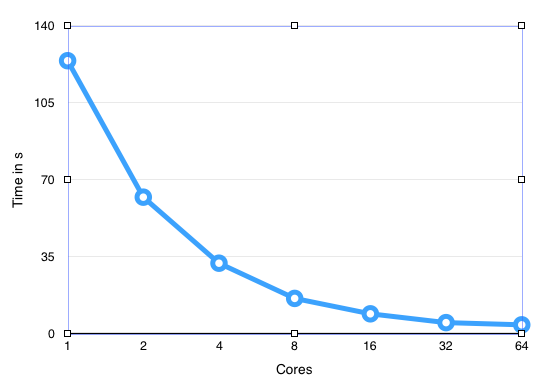
\includegraphics[width=0.75\textwidth]{next_level}
   \caption{Results of the next level bitmap approach.}
   \label{fig:nextbitmap}
\end{figure}

Figure~\ref{fig:nextbitmap} shows the results of the first version of our algorithm. There is a quite good speedup with a higher number of cores, but the problem, like mentioned in Section~\ref{sec:firstversion}, is that we do not have a parent array at the end of this algorithm and it is hard to extend this approach to get one.

\subsection{Testing the second version}

\begin{figure}[!ht]
   \centering
   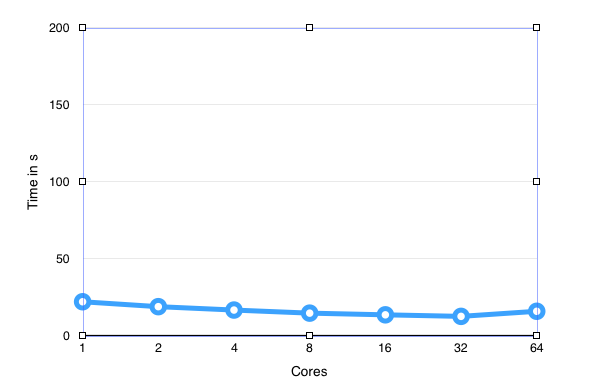
\includegraphics[width=0.75\textwidth]{parent_array}
   \caption{Results of the next level array approach.}
   \label{fig:parentarray}
\end{figure}

Figure~\ref{fig:parentarray} illustrates the results of the second version. As we can see this solution has a very bad speedup with the raising number of cores. Reason for that bad speedup is the reduce scatter operation. It takes too much time to reduce the entries of the next level array with the MAX operation. In Table~\ref{tab:reducescatter} it is shown how much time the reduce scatter operation consumes for the different count of cores.

\begin{table}[!ht]
	\centering
	\begin{tabular}{ | l | l |}
  		\hline
  		Number of Cores & Time for reducing \\ \hline
  		1 & 3.41s \\ \hline
		2 & 9.61s \\ \hline
		4 & 10.76s \\ \hline
		8 & 11.1s \\ \hline
		16 & 12.0s \\ \hline
		32 & 13.5s \\ \hline
		64 & 14.2s \\ \hline
	\end{tabular}
	\caption{Time for reducing the parent arrays of each core.}
  	\label{tab:reducescatter}
\end{table}

\subsection{Testing the third version}

The third version is a compromise between the first and the second version. On the one hand we want to synchronize as little as possible like in the first version. On the other hand, to get a parent array at the end of the algorithm, we have to synchronize more information than in the first version, but as we see in Figure~\ref{fig:parentarray} reducing the whole next level array of all nodes with the MAX operation is too time-consuming. So we decide to reduce a bitmap of all nodes of the graph with the allreduce operation. Figure~\ref{fig:allvisited} shows the results of this purpose.

\begin{figure}[H]
   \centering
   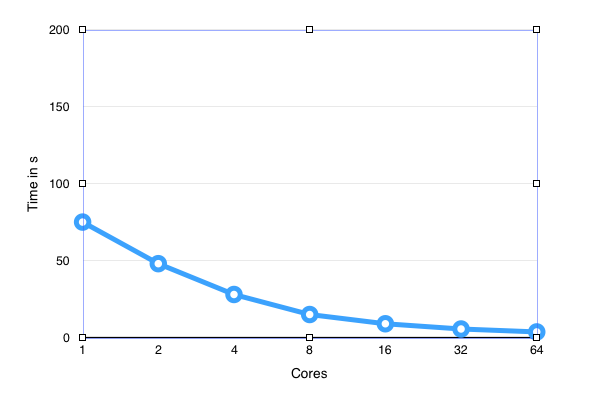
\includegraphics[width=0.75\textwidth]{allvisited}
   \caption{Results of the third and current version.}
   \label{fig:allvisited}
\end{figure}

CALCULATION OF SPEEDUP FOLLOWS!!!

\section{The graph500 project and my own realisation}
\label{sec:graph500}

The graph500 \cite{graph500} is a benchmark of supercomputer systems and concentrates on data intensive loads. Instead of counting double precision floating-point, the benchmark stresses more the communication between the nodes of the system. There are two kernels in this benchmark which are important for the computation and are timed. The first kernel has to generate a graph from the given edge list. In the second kernel is a computation of the parent array of a given search key. This computation is done by a BFS search on the graph generated in the first kernel and is repeated 64 times each time with a new randomly sampled search key.\\
\\
\begin{listing}[H]
\begin{ccode}
/*
input: scale and edgefactor
output: performance information
*/
void graph500_benchmark(scale, edgefactor){
	edge_list = generate_edges(scale, edgefactor);
	buffer = kernel_1(edge_list, pow(2,scale)*edgefactor); // timed
	keys = generate_keys(scale, 64);
	performance_information = kernel_2(buffer); // timed
	print(performance_information);
}
\end{ccode}
\caption{Graph500 benchmark in pseudo code.}
\label{lst:graph500}
\end{listing}

Before the first kernel starts there is a generation of the edge list with a Kronecker generator, as illustrated in Listing~\ref{lst:graph500} through \cinline/edge_list = generate_edges(scale, edgefactor);/. The most important thing in this function is that there is a generation of undirected edge tuples which must not show any locality that can be exploited by the timed kernels. Our implementation of the Kronecker generator takes the two parameters \(scale\) and \(edgefactor\) and has the initiator parameters specified in Table~\ref{tab:kronecker}.\\
\begin{table}[h]
	\centering
	\begin{tabular}{ | l | r |}
  		\hline
  		0.57 & 0.19 \\ \hline
  		0.19 & 0.05 \\ \hline
	\end{tabular}
	\caption{Initiator parameters for the Kronecker generator}
  	\label{tab:kronecker}
\end{table}
That means that each edge has a specific probability to belong to the corresponding quarter of the adjacency matrix. This procedure needs some iterations, more precisely \(scale\) iterations to generate one edge.
After that the computation of the graph, which is later used in kernel 2, follows.
\begin{ccode}
buffer = kernel_1(edge_list, pow(2,scale)*edgefactor);
\end{ccode}
This step is timed, so it is important that it is done as fast as possible. But the fastest solution is not always the best one, because the computed graph from kernel 1 must be also useable for kernel 2 in an appropriate way.\\
Our solution for kernel 1, shown in Listing~\ref{lst:kernel1}, is that we sort the edge list ascending by vertex identifier, first by the start vertex identifier second by the end vertex identifier. //FIGURE FROM SORTING
\begin{listing}[H]
\begin{ccode}
/*
input: edge list and count of edges
output: buffer and scale
*/
int kernel_1(edge_list, edges, *buffer){
	scatter(edge_list); // before sorting the edge list is scattered
	sort(edge_list);
	tree_merge(edge_list); //the sorted edge list is merged in a tree based way
	if (rank == root){
		scale = calculate_scale(edge_list);
	}
	bcast(scale); // scale is broadcasted
	bounds = calculate_bounds(edge_list);
	scatter(bounds);
	scatter(edge_list); //now the sorted edge list is scattered
	buffer = create_buffer(edge_list); //each proc creates the buffer from the received edge list
	return scale;
}
\end{ccode}
\caption{Kernel 1}
\label{lst:kernel1}
\end{listing}
The sorting of the edge list is done in parallel with a quicksort merge implementation to get a good performance for the first kernel. We choose the sorting algorithm quicksort, because it is a efficient sorting algorithm, particularly and that is important, in average case. The procedure is to scatter the edge list to the processors and every processor does the quicksort on the received edge list. The next step is to merge the different sorted edge lists in a way, that the root processor has the whole sorted edge list at the end. Instead of calling the merge operation \(p\) times in sequential order, where \(p\) is the count of processors, we decided to implement a tree based merging of the edge lists, like Puneet Kataria presented in his work \cite{quickmerge}. FIGURE\\\\
With the sorted and merged edge list the \(scale\) or rather the count of nodes is calculated at the root processor and the the edge list is scattered again to the processors. Every processor gets the edges of the nodes he owns, what is guaranteed with \cinline/bounds = calculate_bounds(edge_list);/ . For instance if we have 64 nodes and four processors then the first processor gets the edges with the start vertex from 0 to 15. The second processor gets the edges from 16 to 31, the third from 32 to 47, the last from 48 to 63. So the processors can get a different count of edges, dependent on the start vertex of the edges. We first send the processors the count of the specific edges with \cinline/scatter(bounds);/. Then the processor allocates memory for that edges and receives them. \\
With the splitted edge list the buffer, which will be used in kernel 2, is created in such a way that the buffer contains the end vertex entries of the received edges. Duplicate edges are eliminated. To know at which entry the edges of each node start, we need an additional array of the size of owned nodes. With that the first kernel is completed. // FIGURE \\
\begin{listing}[H]
\begin{ccode}
/*
input: buffer 
output: performance information
*/
char *kernel_2(buffer){
	keys = generate_keys(scale, 64);
	for each(Key k : keys){
		parent_array = BFS(buffer, k); // timed
		validate(parent_array);
	}
}
\end{ccode}
\caption{Kernel 2}
\label{lst:kernel2}
\end{listing}
For the second kernel, as illustrated in Listing~\ref{lst:kernel2}, there have to be a BFS search of 64 keys, which are randomly sampled. Firstly we generate the search keys with 
\begin{ccode}
keys = generate_keys(scale, 64);
\end{ccode}
Secondly we iterate over them and compute a parent array for earch search key \cinline/k/ with
\begin{ccode}
parent_array = BFS(buffer, k);
\end{ccode}
For the BFS search we use our solution from Section~\ref{sec:core} or rather~\ref{sec:thirdversion}. To know if the computed parent array is correct, there is a validation after each BFS search. This validation is not timed and doesn't influences the performance output, so it is sequential in our solution.\\
Further informations and code details of our solution of the graph500 benchmark can be found in Appendix~\ref{sec:sourcecode}.

\section{Graph500 performance of Jupiter}
\label{sec:performance}

The performance of Jupiter is measured by Kernel 1, where the graph is generated from the input edge list, and Kernel 2, where 64 parent arrays are computed within a BFS search. Figure~\ref{fig:kernel1} shows the execution times in seconds of the first kernel from a scale of nodes from 24 to .... and an edgefactor of 16 with 1 core up to 512 cores.


In contrast Kernel 2 is measured by the performance metric TEPS (traversed edges per second).  Let \(m\) be the number of input edge tuples within the component traversed by the search and \(t(n)\) be the execution time for Kernel 2. Then the normalized performance rate is: \(TEPS(n) = m / t(n)\)\\
Figure~\ref{fig:kernel2} shows the TEPS with a scale of 24 and an edgefactor of 16 with different counts of computing cores.

\section{Why no parallel realisation of depth-first search?}
\label{sec:depth-first search}

\section{Summary}
\label{sec:summary}

\clearpage

\nocite{*}
\bibliographystyle{abbrv}
\bibliography{bachelor}
\clearpage
\appendix
\section{BFS versions}
\label{sec:versions}
Bla bla
\section{Source Code - graph500}
\label{sec:sourcecode}
\lstinputlisting[caption={BFS solution},label=bfs]{../Source/bfs_par_allvisited_parallelsort.c}
\clearpage
\lstinputlisting[caption={Kronecker Generator},label=kronecker_generator]{../Source/kronecker_generator.c}
\clearpage
\lstinputlisting[caption={project.h},label=project]{../Source/project.h}

\clearpage


\end{document}